% Drawing 85/02-2 -- folder 85, batch 02, archive page 34 (PDF page 35).
% Transcription: à gauche, en marge, un dessin : une étoile de huit arêtes courbes issues d'un sommet, chacune terminée par un point
% Kind: star of eight edges from one vertex. Method 2 (schematic redraw from the facsimile). Status: ok.
% Notes: Ink. Eight curved edges from one centre, each ending at a dot; all start at the same point. Redrawn 2026-11-12 (issue 128): to check again.
% Coordinates: 1 unit = 1 mm = 1/100 of the crop width (bbox in page fractions: [0.07, 0.18, 0.25, 0.31]).
% Redrawn by Claude (claude-fable-5-2), issue #128, 2026-11-12; not checked by a human; not compiled (no TeX in the session).
% Rights: reproduces part of the work -- behind RENDER_TRANSCRIPTS, never published by itself.
\documentclass[tikz,border=3pt]{standalone}
\usepackage{amsmath,amssymb}
\usetikzlibrary{patterns,arrows.meta}
\tikzset{pencil/.style={black!45}, struck/.style={black!35}, mpt/.style={circle,draw,inner sep=1.3pt}, pt/.style={circle,fill,inner sep=0.9pt}, opt/.style={circle,draw,fill=white,inner sep=1.1pt}}
\begin{document}
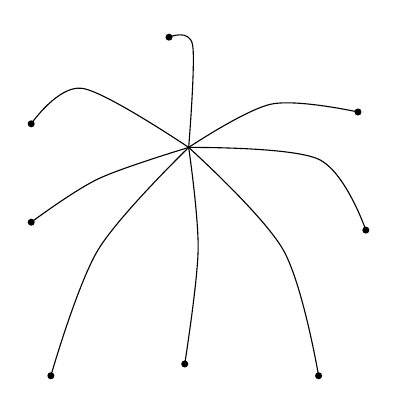
\begin{tikzpicture}[x=1mm,y=1mm,line cap=round,line join=round,font=\scriptsize]
\draw plot[smooth, tension=0.55] coordinates {(44.5,-39) (31,-31.5) (24.5,-36)};
\draw plot[smooth, tension=0.55] coordinates {(44.5,-39) (45,-26) (42,-25)};
\draw plot[smooth, tension=0.55] coordinates {(44.5,-39) (55,-33.5) (66,-34.5)};
\draw plot[smooth, tension=0.55] coordinates {(44.5,-39) (61,-40.5) (67,-49.5)};
\draw plot[smooth, tension=0.55] coordinates {(44.5,-39) (56.5,-52) (61,-68)};
\draw plot[smooth, tension=0.55] coordinates {(44.5,-39) (45.7,-52) (44,-66.5)};
\draw plot[smooth, tension=0.55] coordinates {(44.5,-39) (33,-52) (27,-68)};
\draw plot[smooth, tension=0.55] coordinates {(44.5,-39) (33,-43) (24.5,-48.5)};
\node[pt] at (24.5,-36) {};
\node[pt] at (42,-25) {};
\node[pt] at (66,-34.5) {};
\node[pt] at (67,-49.5) {};
\node[pt] at (61,-68) {};
\node[pt] at (44,-66.5) {};
\node[pt] at (27,-68) {};
\node[pt] at (24.5,-48.5) {};
\end{tikzpicture}
\end{document}
